\documentclass[conference]{IEEEtran}
\usepackage[utf8]{inputenc}
\usepackage[T1]{fontenc}
\usepackage{graphicx}
\usepackage{booktabs}
\usepackage{siunitx}
\usepackage{url}
\usepackage{hyperref}
\hypersetup{colorlinks=true,linkcolor=black,citecolor=black,urlcolor=blue}
\graphicspath{{figures/}}

\title{A Low-Cost Networked Acoustic and Vibration Sensor Node for Early Detection of Insects in Bagged Rice}

\author{\IEEEauthorblockN{Dilan Perera}
\IEEEauthorblockA{Intelligent Systems \& Mechatronics Research Laboratory (ISMR Labs)\\
Colombo, Sri Lanka\\
\url{https://github.com/ISMR-Labs/grain-acoustics}}}

\begin{document}
\maketitle

\begin{abstract}
Stored-product insects infest retail rice bags long before damage is visible from outside the bag. Acoustic detection of hidden insects in grain is well established with laboratory-grade sensors, but no cheap networked sensor exists that a warehouse could attach to a bag. This paper describes the design and first characterisation of such a node. An ESP32 microcontroller samples two I2S MEMS microphones at \SI{16}{kHz} and two bare piezoelectric contact discs at \SI{8}{kHz} and streams every sample over Wi-Fi in \SI{100}{ms} HTTP chunks (about \SI{104}{kB/s}) to a self-hosted server that visualises the four channels live, records sessions as WAV with metadata, and exports every channel separately. We report the hardware, firmware and protocol, two problems met during bring-up (a second microphone that cannot share the I2S data line, and the loss of DMA ADC sampling once both I2S peripherals are taken) and their solutions, and a baseline characterisation of the four channels. The microphones reach a noise floor of \SIrange{-26}{-32}{dBFS} and agree within \SI{1}{dB}. The bare piezo channels are dominated by \SI{50}{Hz} mains pickup \SI{30}{dB} above the surrounding spectrum and clip on 7--15\,\% of samples, so a charge amplifier and shielded leads are required before insect trials. The complete design, recordings and analysis scripts are published as an open repository.
\end{abstract}

\begin{IEEEkeywords}
stored-product insects, acoustic detection, biotremology, piezoelectric sensor, MEMS microphone, ESP32, rice
\end{IEEEkeywords}

\section{Introduction}
Rice is sold in Sri Lanka in \SI{5}{kg} retail bags that are stacked in warehouses for weeks. A few adult rice weevils (\emph{Sitophilus oryzae}), lesser grain borers (\emph{Rhyzopertha dominica}) or red flour beetles (\emph{Tribolium castaneum}) in a sealed bag are invisible, and by the time frass or holes appear the whole stack is affected. Insects inside grain are not silent: feeding, chewing and walking produce trains of short broadband impulses that propagate as airborne sound and as substrate vibration through the packed kernels \cite{mankin2011,hill2016}. Acoustic detection of hidden stored-grain insects has been demonstrated since the early 1990s with probe sensors and laboratory amplifiers \cite{hagstrum1993,shuman1993}, has been automated with pattern recognition \cite{potamitis2009,eliopoulos2015}, and recent reviews point to low-cost microcontroller platforms as the next step \cite{mankin2021}. Contact piezo microphones in 3D-printed housings have also been shown to be adequate for biotremology of small insects \cite{gjonov2025}.

This work asks three questions. (1) Can a low-cost MEMS microphone and a bare piezo disc coupled to a sealed bag capture insect signals above the warehouse noise floor? (2) Which coupling, airborne, contact on the bag wall, or probe in the grain, gives the best signal-to-noise ratio for the smallest insects? (3) Can the resulting recordings train a detector that flags an infested bag early? This paper covers the platform built to answer them and its baseline characterisation; insect trials are future work.

\section{System Design}

\subsection{Sensor node}
The node (Fig.~\ref{fig:hw}) is built around an ESP32-WROOM-32U development board with an external \SI{2.4}{GHz} antenna. Two INMP441 I2S MEMS microphones \cite{inmp441} provide the airborne channels and two \SI{27}{mm} brass piezo discs the contact channels. The discs are used bare, without an amplifier, as a deliberate first pass to establish what the ADC alone can resolve. Each disc feeds an ESP32 ADC pin through \SI{100}{k\ohm}, with a \SI{1}{M\ohm} load to a \SI{0.55}{V} bias node and a BAT54S Schottky pair clamping knocks to the rails. The ADC runs at \SI{0}{dB} attenuation (\SIrange{0}{1.1}{V} window), so one count is about \SI{0.27}{mV} at the pin.

Table~\ref{tab:pins} lists the pin assignment. Each microphone has its own I2S peripheral; the reason is discussed in Section~\ref{sec:bringup}.

\begin{table}[t]
\caption{Sensor node pin map}
\label{tab:pins}
\centering
\begin{tabular}{lll}
\toprule
ESP32 pin & Function & Connection \\
\midrule
GPIO 26 / 25 / 33 & I2S1 BCLK / WS / DIN & Mic A SCK / WS / SD \\
GPIO 14 / 27 / 32 & I2S0 BCLK / WS / DIN & Mic B SCK / WS / SD \\
GPIO 34 & ADC1 ch 6 & Piezo 1 network \\
GPIO 35 & ADC1 ch 7 & Piezo 2 network \\
GPIO 4 & output & status LED \\
3V3 / GND & power & mics, bias divider, clamps \\
\bottomrule
\end{tabular}
\end{table}

\begin{figure}[t]
\centering
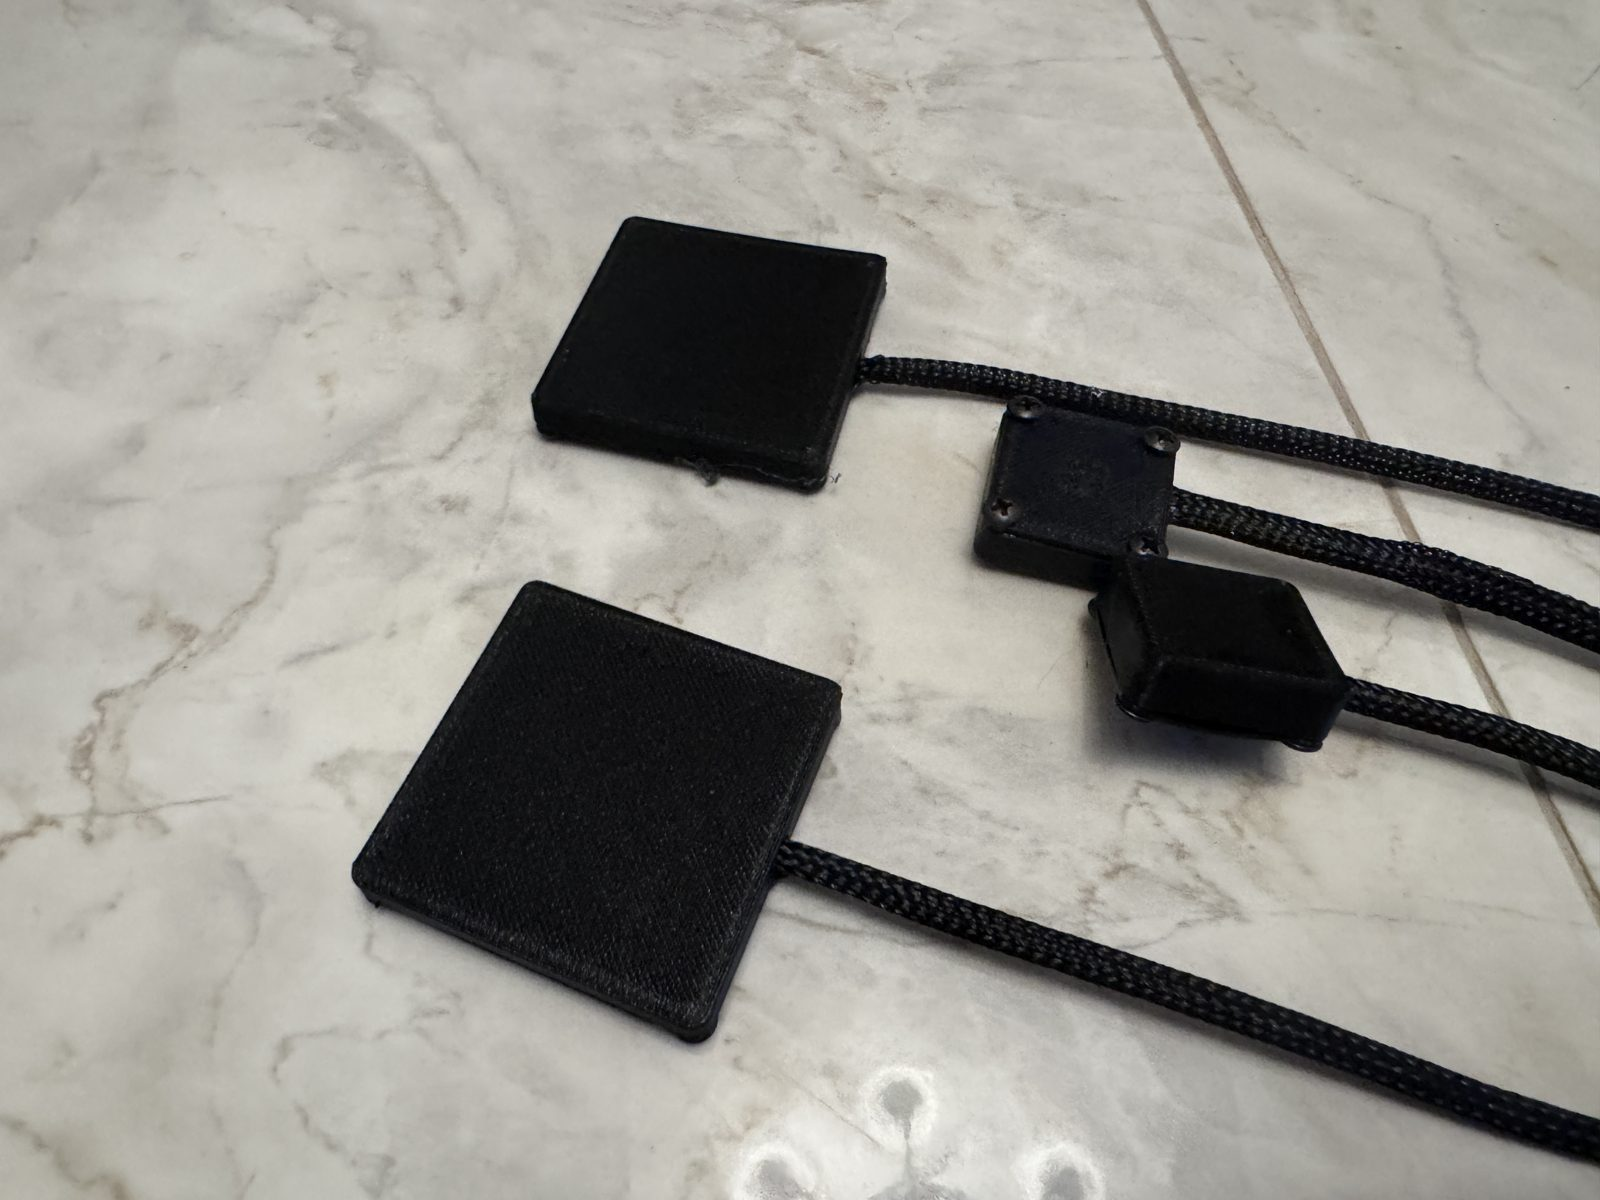
\includegraphics[width=\columnwidth]{node-hardware.jpg}
\caption{The node: controller box with four cable glands, two \SI{57}{mm} piezo pads and two \SI{30}{mm} microphone pods, all 3D-printed in PLA+.}
\label{fig:hw}
\end{figure}

\subsection{Enclosures}
Three enclosures were designed in OpenSCAD and printed on a Creality Ender-3 V3 SE: a controller box (inner $20\times70\times40$\,mm, USB-C cutout, four \SI{4}{mm} cable glands), a microphone pod ($30\times30\times8.7$\,mm, four-hole grille), and a piezo pad ($57\times57\times5.5$\,mm, \SI{3}{mm} cavity, \SI{2}{mm} contact floor) modelled on the contact microphone box of \cite{gjonov2025}. Walls are \SI{1.35}{mm}, exactly three extrusion lines, so the slicer produces clean perimeters around the cable holes.

\subsection{Firmware}
The firmware runs on Arduino-ESP32 3.3 over ESP-IDF~5. Two independent I2S standard-mode receive channels capture 32-bit Philips stereo frames at \SI{16}{kHz}; the left slot is kept and bits 29..14 of the 24-bit sample become an \texttt{int16}. To keep both DMA rings small (4~descriptors of 256 frames) each \SI{100}{ms} chunk is read in two \SI{50}{ms} halves per microphone. The piezos are sampled by a \SI{1}{MHz} hardware timer whose interrupt notifies a high-priority FreeRTOS task; the task performs two one-shot ADC conversions per tick into a ring buffer. The measured rate is \SIrange{7987}{8013}{Hz}. A queue of six chunk buffers decouples capture from an HTTP task that POSTs each chunk with keep-alive; if Wi-Fi stalls, chunks are dropped rather than delayed, and the server zero-fills the gap so recordings remain on a continuous time axis. Over-the-air updates are supported.

\subsection{Protocol and server}
Each chunk carries a 32-byte little-endian header (magic \texttt{SNS1}, sequence number, uptime, both sample rates, frame counts, flags) followed by interleaved \texttt{int16} microphone samples and interleaved \texttt{uint16} raw ADC counts. The server is a FastAPI application in Docker behind a TLS reverse proxy. It fans chunks out to browser clients over WebSocket through bounded per-client queues, writes recordings as \texttt{mics.wav} (2~ch, \SI{16}{kHz}) and \texttt{piezo.wav} (2~ch, \SI{8}{kHz}, ADC $-$ 2048) with a JSON sidecar, and exports each channel as a mono WAV. The dashboard (Fig.~\ref{fig:dash}) shows four oscilloscopes with live spectra, RMS and peak levels, a record button and a recordings table with one download link per channel. A \SI{0.4}{s} jitter buffer keeps the display smooth at \SI{30}{fps}.

\begin{figure}[t]
\centering
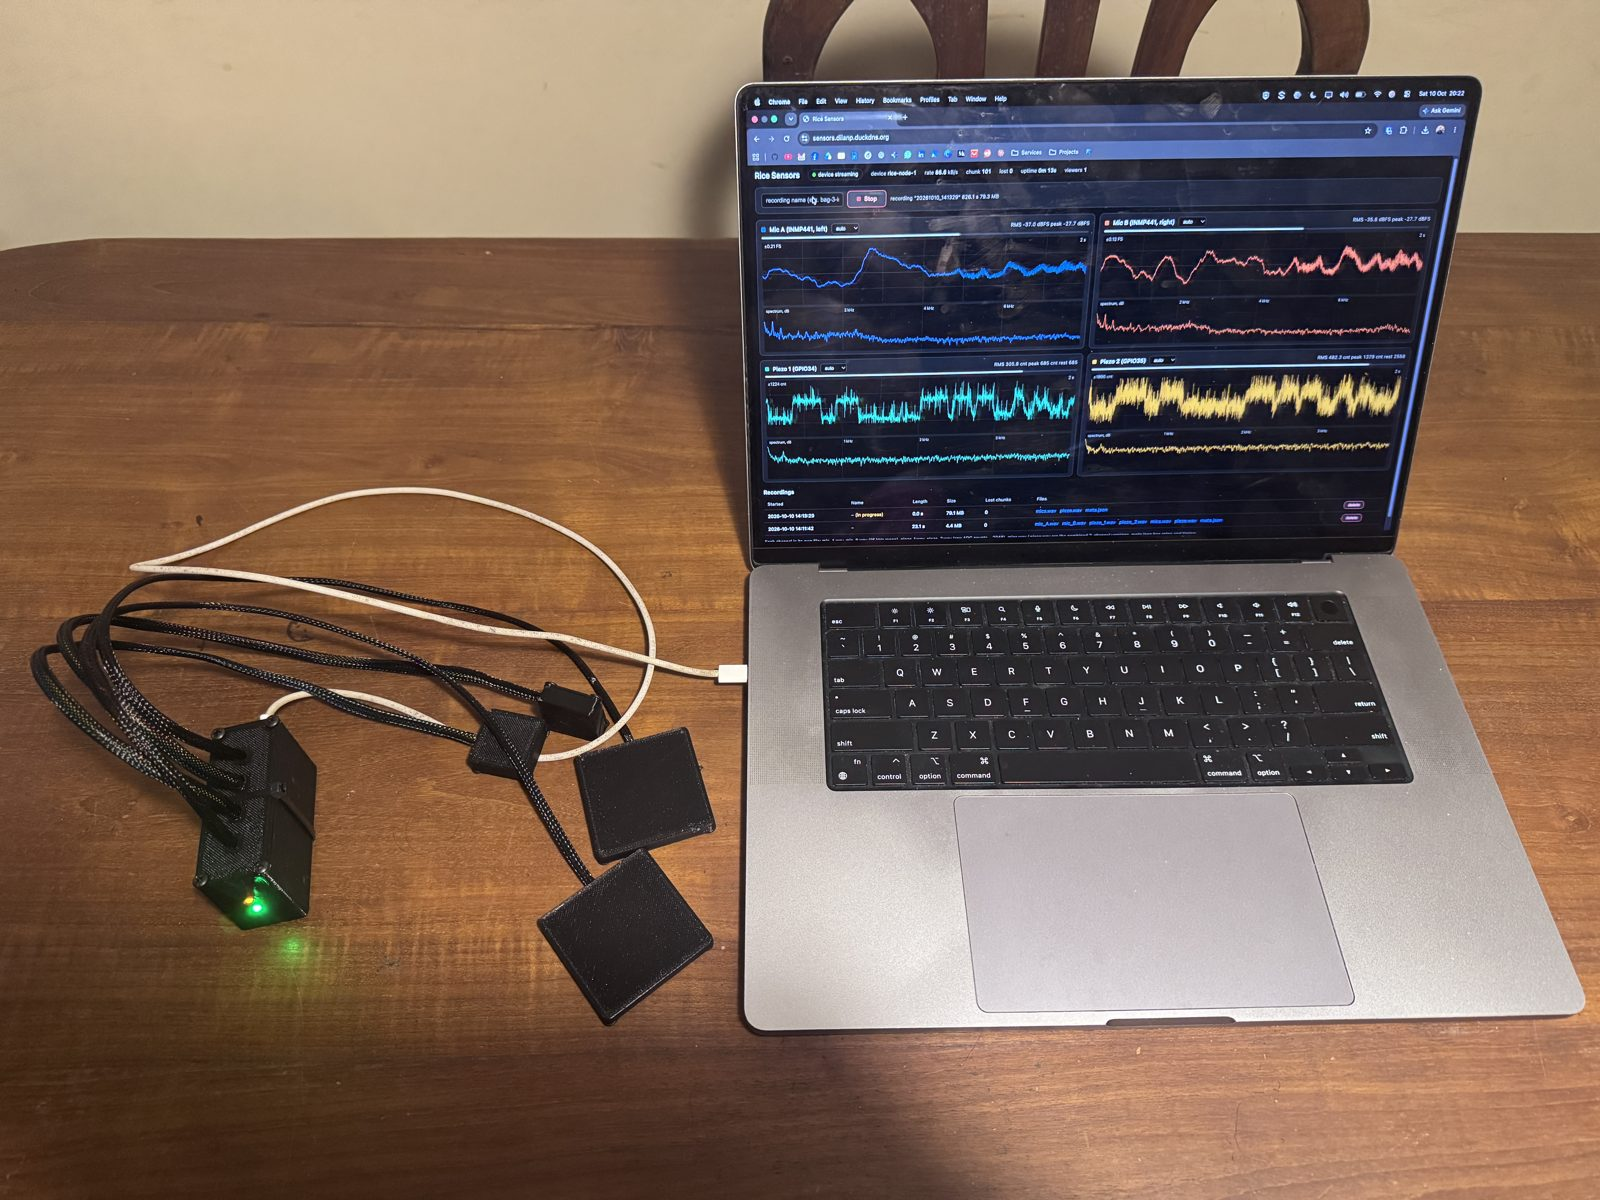
\includegraphics[width=\columnwidth]{node-dashboard.jpg}
\caption{Node streaming to the live dashboard: two microphone scopes (top) and two piezo scopes (bottom), each with its spectrum.}
\label{fig:dash}
\end{figure}

\section{Bring-up Problems and Solutions}
\label{sec:bringup}

\subsection{Second microphone on a shared data line}
The INMP441 is designed so that two devices share one data line, one per stereo slot, selected by the L/R pin. In our build the second microphone never drove the line, and whenever it was connected the first microphone's stream was corrupted: 74\,\% zero samples with a \SI{640}{ms} periodic bit pattern. Swapping modules, pins and L/R ties did not change the symptom. Moving Mic~B to the ESP32's second I2S peripheral (I2S0) on its own three pins fixed both faults at once (Fig.~\ref{fig:micb}). The second \texttt{i2s\_new\_channel} call initially failed to allocate DMA memory; reducing the DMA ring to 4$\times$256 frames per channel and reading in halves resolved it.

\begin{figure}[t]
\centering
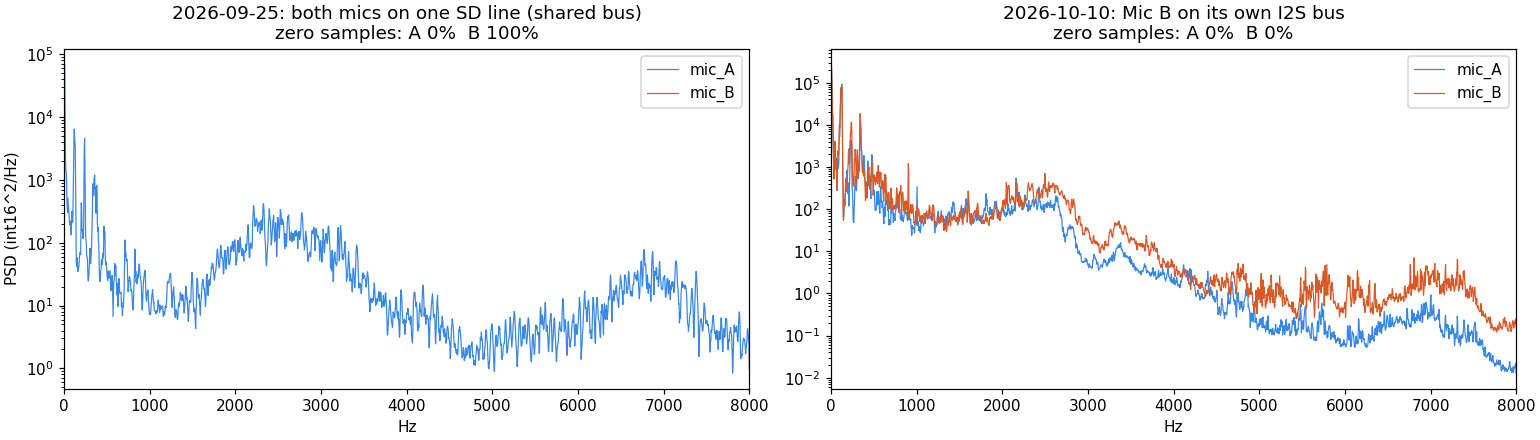
\includegraphics[width=\columnwidth]{micB_shared_vs_separate_bus.png}
\caption{Power spectral density of both microphones before (left, shared data line, Mic~B 100\,\% zeros) and after (right, separate buses) the change.}
\label{fig:micb}
\end{figure}

\subsection{Loss of DMA ADC sampling}
On the classic ESP32 the continuous (DMA) ADC driver borrows the I2S0 peripheral. Once Mic~B occupied I2S0, DMA sampling of the piezos became impossible. The timer-plus-task design in the firmware section replaced it; the cost is \SI{0.3}{\percent} rate jitter, which the server tolerates by trusting the per-chunk frame count rather than a nominal rate.

\section{Baseline Characterisation}
Two sessions recorded on 10~October~2026 with the final wiring were analysed with the repository's \texttt{spectrogram.py} (Welch PSD, 4096-point segments). Session~A (\SI{23.1}{s}) included deliberate handling, taps and speech near the sensors; Session~B (\SI{8.2}{s}) was a quiet bench with the node resting on a table. Table~\ref{tab:levels} summarises the levels and Fig.~\ref{fig:overview} shows Session~A.

\begin{table}[t]
\caption{Channel levels (0~dBFS = ADC or int16 full scale)}
\label{tab:levels}
\centering\footnotesize
\setlength{\tabcolsep}{4pt}
\sisetup{table-format=-2.1}
\begin{tabular}{llSSSS}
\toprule
Sess. & Channel & {RMS} & {Peak} & {Clip \%} & {50 Hz} \\
 & & {dBFS} & {dBFS} & & {excess dB} \\
\midrule
A & mic A   & -22.5 & -5.9 & 0.0 & 1.9 \\
A & mic B   & -23.1 & -1.9 & 0.0 & 0.9 \\
A & piezo 1 & -12.9 &  0.0 & 0.0 & -0.9 \\
A & piezo 2 & -12.8 & -1.8 & 0.0 & -0.7 \\
B & mic A   & -26.4 & -16.5 & 0.0 & -4.9 \\
B & mic B   & -31.7 & -19.7 & 0.0 & -3.3 \\
B & piezo 1 & -5.0 &  0.0 & 6.9 & 30.7 \\
B & piezo 2 & -3.6 &  0.0 & 15.5 & 31.6 \\
\bottomrule
\end{tabular}
\end{table}

\begin{figure*}[t]
\centering
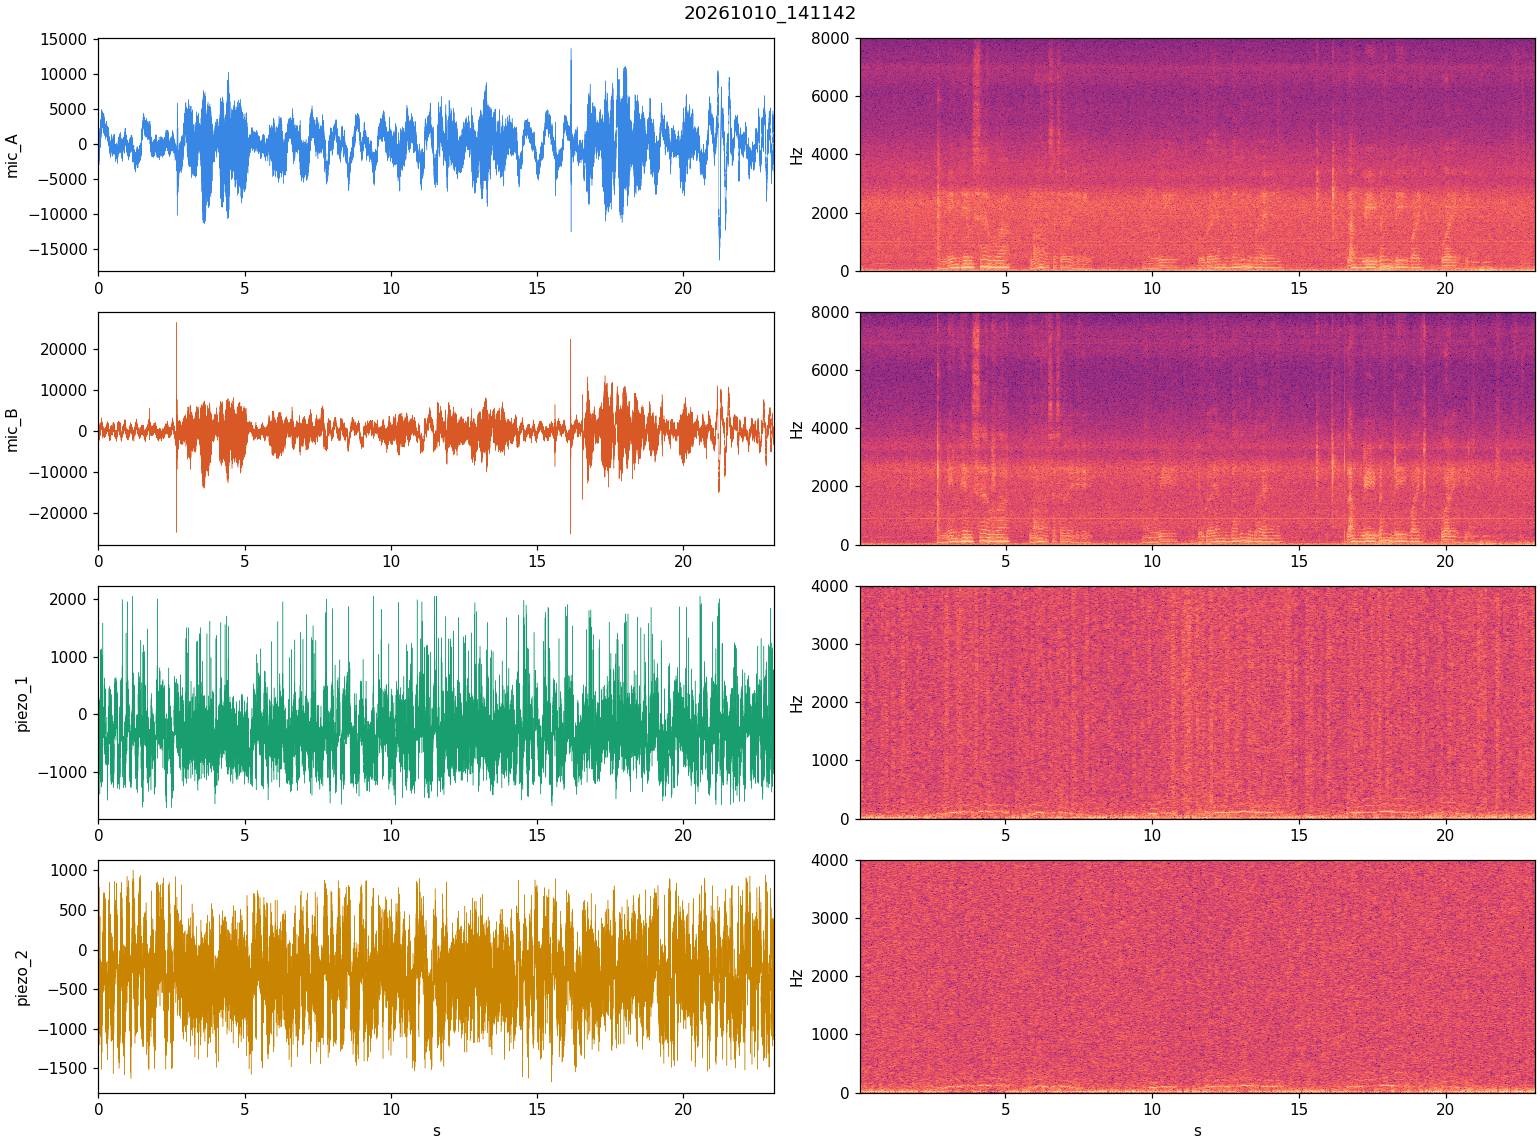
\includegraphics[width=\textwidth]{20261010_141142_overview.png}
\caption{Session A: waveforms (left) and spectrograms (right) of both microphones (\SI{16}{kHz}) and both piezo channels (\SI{8}{kHz}). Speech and handling are visible on the microphones; the piezo channels show broadband noise and a \SI{50}{Hz} line.}
\label{fig:overview}
\end{figure*}

The two microphones agree within \SI{1}{dB} in level and spectrum, and their quiet-bench floor is \SIrange{-26}{-32}{dBFS}, dominated by energy below \SI{100}{Hz} (93--94\,\% of the total), which is room rumble through the table rather than electrical noise. The bare piezo channels behave differently: on the quiet bench the \SI{50}{Hz} mains component sits \SI{31}{dB} above the median of the surrounding band, the RMS level is only \SIrange{4}{5}{dB} below full scale, and 7--15\,\% of samples are clipped. Any insect signal, expected in the tens of microvolts at the bag wall, is far below this floor.

\section{Discussion and Next Steps}
The platform meets its streaming and recording goals: full-rate capture of four channels, lossless accounting of dropped chunks, and per-channel export. The microphone channels are ready for coupling experiments. The piezo channels are not. Three changes are planned before insect trials: shielded leads with the shield grounded at the box, a lower load resistor (\SI{470}{k\ohm}) to reduce hum pickup, and a per-channel LM324 charge amplifier (gain about 1000, \SIrange{300}{5000}{Hz} band-pass) biased to the ADC mid-scale, which needs no firmware change. For mounting, a thin hard bond of the brass face to a stiff metal plate or a probe pushed into the grain is preferred over hot glue on plastic, which damps the \SIrange{1}{5}{kHz} band in which stored-grain insect impulses are reported \cite{mankin2011}.

The experimental plan then follows the literature: a one-hour warehouse baseline on an empty table and on a clean sealed bag; seeded bags with 10, 50 and 200 adult \emph{S.~oryzae} and matched controls, each recorded for \SI{24}{h} with sensors in all four coupling positions, logging temperature because adult activity is strongly temperature dependent \cite{hagstrum1993}; and an impulse-count detector in the style of \cite{shuman1993} as the first classifier.

\section{Conclusion}
A networked four-channel acoustic and vibration sensor node for bagged rice was built from a \SI{5}{USD} microcontroller, two MEMS microphones and two piezo discs, together with a recording platform that exports every channel for analysis. Bring-up showed that two INMP441 microphones should be given separate I2S peripherals on the ESP32, which in turn forces timer-paced ADC sampling. The microphones are quiet and matched; the bare piezo discs need a preamplifier and shielding before they can detect small insects. All hardware designs, firmware, server code, recordings and analysis scripts are available in the project repository \cite{repo}.

\bibliographystyle{IEEEtran}
\bibliography{references}

\end{document}
